\documentclass[10pt]{beamer}
% Class options include: notes, notesonly, handout, trans,
%                        hidesubsections, shadesubsections,
%                        inrow, blue, red, grey, brown

%% \usepackage{beamerthemesplit} 
\usepackage{graphicx}
\graphicspath{{img/}}
\usepackage[utf8]{inputenc}
\usepackage[francais]{babel}
\usepackage[T1]{fontenc}
\usepackage{alltt}
\usepackage{xcolor}
%\usepackage{amssymb}
\usepackage{multicol}
\usepackage{geometry}
%% \usepackage{amsfont}
\usepackage{amsmath}
\usepackage{amssymb}

\newcommand{\bcode}[1]{\textcolor{darkgray}{#1}}
\renewcommand{\ttdefault}{txtt}





\usetheme{CambridgeUS}  


\title[Stage M2]{Traduction de composants Scade/Lustre vers des Machines B}
\author{Florian THIBORD}
\institute{M2-STL APR  /  UPMC}
\date{Année 2012-2013}

\begin{document}

\begin{frame}
  \titlepage
\end{frame}

\begin{frame}
  \tableofcontents
\end{frame}



%% \vspace{1cm}
%%   \uncover<2->{
%%     Présentation d'une nouvelle méthode de résolution du point fixe:\\
%%     Algorithme permettant d'itérer selon une stratégie.
%%   }


\section{Introduction}
\frame{\sectionpage}

\begin{frame}
  \frametitle{Contexte}
Stage réalisé au sein du projet CERCLES$^2$:
Certifier des \textbf{composants} réutilisables à l'aide de \textbf{méthodes
  formelles}.
\vspace{1cm}
\begin{itemize}
  \uncover<2->{
  \item Composant : Programme + \emph{Contrat}
  }
  \uncover<3->{
  \item Méthode Formelle : raisonnement rigoureux sur un composant à l'aide
    d'une logique mathématique.
  }
\end{itemize}
\end{frame}

\begin{frame}
\frametitle{Description du travail}
  Composants développés avec \textbf{Scade}, développé par Esterel
  Technologies:
  \begin{itemize}
  \item Programme écrit avec des schémas-blocs
  \item Engendre du code pseudo-Lustre.
  \end{itemize}
  \vspace{0.7cm}
  \uncover<2->{
    Méthode B, développée par J.R. Abrial, utilisée pour la validation des
    composants:
    \begin{itemize}
    \item Méthode basée sur le \emph{raffinement} de \emph{machines}
    \item Cadre du projet : \textbf{Machine abstraite} raffinée en \textbf{Machine implantation}
    \end{itemize}
  }
  \vspace{0.7cm}
  \uncover<3->{
    Ma tâche : développer un outil permettant de traduire un composant Scade en un
    couple de machines B.
  }
\end{frame}


\begin{frame}
\frametitle{Schéma général}
\begin{figure}[h]
  \begin{center}
    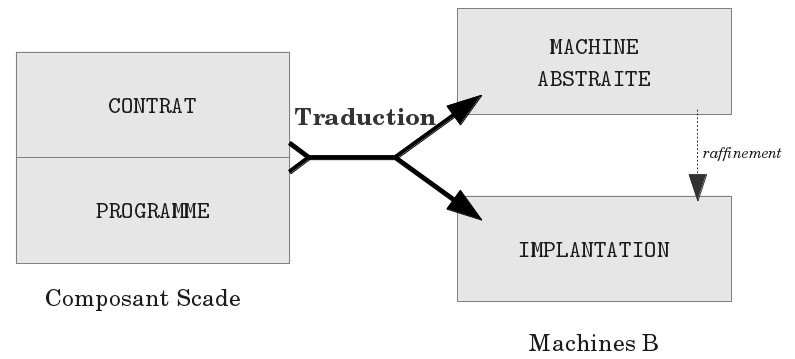
\includegraphics[scale=0.4]{intro_schema2.png}
  \end{center}
\end{figure}
\end{frame}



\section{Scade}
\frame{\sectionpage}

\begin{frame}
\frametitle{Architecture d'un noeud Scade}
Génération de code pseudo-Lustre.
\begin{figure}[h]
  \begin{center}
    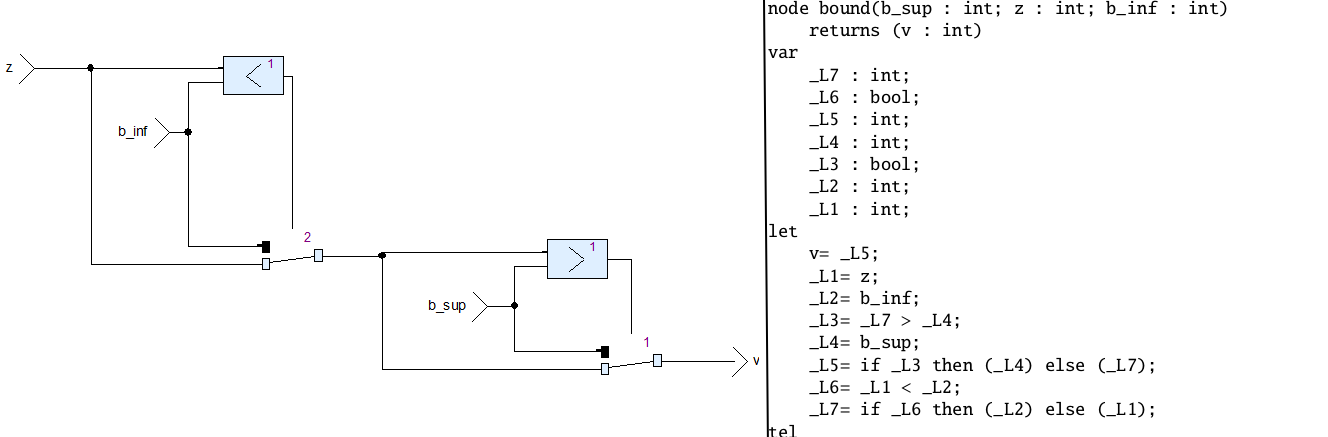
\includegraphics[scale=0.27]{1_ex2.png}
  \end{center}
\end{figure}
Les équations sont atomisées.
\end{frame}


\begin{frame}
\frametitle{Un fragment de Scade}
Le code pseudo lustre est consitué d'un ensemble d'équations atomisées.\\
\vspace{0.7cm}
3 familles d'équations :
\begin{itemize}
\item \texttt{v = op$_{base}$(x$_1$, ..., x$_n$);}
\item \texttt{v = if c then x$_1$ else x$_2$;}
\item \texttt{v$_1$, ..., v$_p$ = op$_{appel}$(x$_1$, ..., x$_n$);}
\end{itemize}
\vspace{0.2cm}
\begin{huge}\begin{center}+\end{center}\end{huge}
\vspace{0.2cm}

1 opérateur particulier: \texttt{fby}. Il prend 3 paramètres : une variable, un délai et une
valeur d'initialisation.

\begin{figure}[h]
\begin{center}
\begin{tabular}{ l || c | c | c | c }
\texttt{instant} & 0 & 1 & 2 & ... \\ \hline
\texttt{v} & 10 & 20 & 30 & ... \\
\texttt{z} & \textbf{0} & 10 & 20 & ... \\
\end{tabular}
\end{center}
\caption{\texttt{z = fby(v, 1, \textbf{0})}}
\end{figure}

\end{frame}


%% \begin{frame}
%% \frametitle{Un langage synchrone}
%% Scade, un langage manipulant des flots de données. A chaque tic d'horloge:
%% \begin{itemize}
%% \item (i) 1 ensemble de flots est reçu en entrée
%% \item (ii) l'ensemble des équations du noeud sont résolues avec (i)
%% \item (iii) le noeud retourne un ensemble de flots correspondants au résultat de (ii)
%% \end{itemize}

%% \vspace{0.6cm}

%% L'opérateur \texttt{fby}, prend 3 arguments : une variable, un délai et une
%% valeur d'initialisation.

%% \begin{figure}[h]
%% \begin{center}
%% \begin{tabular}{ l || c | c | c | c }
%% \texttt{instant} & 0 & 1 & 2 & ... \\ \hline
%% \texttt{v} & 10 & 20 & 30 & ... \\
%% \texttt{z} & 0 & 10 & 20 & ... \\
%% \end{tabular}
%% \end{center}
%% \caption{\texttt{z = fby(v, 1, 0)}}
%% \end{figure}
%% \end{frame}

\begin{frame}
\frametitle{Contrat avec Scade}
  Assertions écrites manuellement dans Scade. Elles sont de 2 type:
\begin{itemize}
\item \texttt{assume A : expr} où expr correspond à une condition sur une entrée
\item \texttt{guarantee G : expr} où expr correspond à une condition sur une sortie
\end{itemize}
  \vspace{0.4cm}
\uncover<2->{
  Exemple sur le noeud \texttt{Bound}:\\
  \vspace{0.4cm}
  \begin{footnotesize}
    \begin{semiverbatim}
      assume A\_1 : b\_inf <= 2000 and b\_inf >= -2000;

      assume A\_2 : b\_sup <= 2000 and b\_sup >= -2000;

      assume A\_3 : z <= 2000 and z >= -2000;

      guarantee G\_1 : v <= 2000 and v >= -2000;
    \end{semiverbatim}
  \end{footnotesize}
}
\end{frame}




\section{Machines B}
\frame{\sectionpage}
\begin{frame}

Les machines sont organisées en \emph{clauses}.
\setlength{\columnseprule}{0.05cm}
\begin{scriptsize}
\begin{multicols}{2}
\begin{center}\emph{MACHINE ABSTRAITE}\end{center}
\begin{semiverbatim}
\textbf{MACHINE} Ma\_machine


\textbf{OPERATIONS}

 ...\uncover<2->{\emph{Substitutions}}

\textbf{END}
\end{semiverbatim}

\columnbreak
\begin{center}\emph{IMPLANTATION}\end{center}
\begin{semiverbatim}
\textbf{IMPLEMENTATION} Ma\_machine\_i

\textbf{REFINES} Ma\_machine

\textbf{IMPORTS} ...\uncover<2->{\emph{Déclarations machines}}

\textbf{CONCRETE\_VARIABLES} ...\uncover<2->{\emph{Déclaration variables}}

\textbf{INVARIANT}

  ...\uncover<2->{\emph{Prédicat}}

\textbf{INITIALISATION}

  ...\uncover<2->{\emph{Substitutions}}

\textbf{OPERATIONS}

  ...\uncover<2->{\emph{Substitutions}}

\textbf{END}
\end{semiverbatim}
\end{multicols}
\end{scriptsize}

\uncover<2->{
  Le langage B est un langage ensembliste.\\
  Les substitutions généralisées permettent de transformer les prédicats.
}

\end{frame}


%% \begin{frame}
%%   \frametitle{Substitutions Généralisées}
%%  Elles permettent de transformer les prédicats.

%% \vspace{0.5cm}

%% \textbf{Devient Egal} : [ x:=e ] P \\
%% Occurences libres de x dans P remplacées par e.

%% \vspace{0.3cm}
%% \textbf{Appel Opération} : [R $\leftarrow$ op(E)]P\\
%% Instanciation de l'opération op avec E comme paramètre.

%% \vspace{0.3cm}
%% \textbf{Condition} : [IF P THEN S ELSE T]R \\
%% Alternative.

%% \vspace{0.3cm}
%% \textbf{Définition de Variable Locale} : [VAR X IN S END]  \\
%% Les variables X sont accessibles dans S.

%% \vspace{0.3cm}
%% \textbf{Devient Element De} : [X:$\in$ E] \\
%% Substitution indéterminée attribuant à X une valeur tirée dans E.

%% \vspace{0.3cm}
%% \textbf{Precondition} : [PRE P THEN S END]\\
%% Fixe les préconditions P sous lesquelles S sera valide.

%% \end{frame}

\begin{frame}
\frametitle{Exemple}
\begin{scriptsize}
\setlength{\columnseprule}{0.05cm}
\begin{multicols}{2}
\begin{semiverbatim}
\textbf{MACHINE} Integr


\textbf{OPERATION}

yy $\leftarrow$ integr(xx) =

  \textbf{PRE}

$~~$    xx $\in$ INT \& -256 <= xx \& xx <= 255

  \textbf{THEN}

$~~$    yy $\in$: \{ ii | ii $\in$ INT \& 

$~~$$~~$          -1024 <= ii \& ii <= 1023\}

  \textbf{END}
\end{semiverbatim}

\columnbreak

\begin{semiverbatim}
\textbf{IMPLEMENTATION} Integr\_i

\textbf{REFINES} Integr

\textbf{IMPORTS} Bound

\textbf{CONCRETE\_VARIABLES} reg1

\textbf{INVARIANT}

$~$  reg1 $\in$ INT \& -1024 <= reg1 \& reg1 <= 1023

\textbf{INITIALISATION}

$~$  reg1 := 0


\textbf{OPERATIONS}


yy $\leftarrow$ integr(xx) =

\textbf{VAR} zz \textbf{IN}

$~~$   zz := xx + reg1; 

$~~$   yy $\leftarrow$ bound(-1024, zz, 1023);

$~~$   reg1 := yy

\textbf{END}
\end{semiverbatim}
\end{multicols}
\end{scriptsize}

\uncover<2->{
  Chaque étape de raffinement engendre des obligations de preuves.
}

\end{frame}



\section{Schémas de traduction}
\frame{\sectionpage}
\subsection{Machine Abstraite}

%% \begin{frame}
%% \frametitle{Traduction des déclarations}

%% \begin{small}La déclaration de noeud Scade suivante :\end{small}
%% \begin{semiverbatim}
%% \begin{scriptsize}
%% node mon\_noeud 
%%  (in$_1$: type\_in$_1$, ..., in$_n$: type\_in$_n$ ) 

%% $~~$returns 

%% $~~$(out$_1$: type\_out$_1$, ..., out$_m$: type\_out$_m$);
%% \end{scriptsize}
%% \end{semiverbatim}
%% \begin{small}
%% Traduction vers la déclaration d'opération B:
%% \end{small}
%% \begin{semiverbatim}
%% \begin{scriptsize}
%% \color{darkgray}
%% in$_1$, ..., in$_n$ $\leftarrow$ mon\_noeud(out$_1$, ..., out$_m$) =
%% \end{scriptsize}
%% \end{semiverbatim}
%% \end{frame}

\begin{frame}

\frametitle{Traduction des conditions}
Utilisation d'une substitution \emph{Precondition} PRE \textbf{P} THEN
\textbf{S} END:
\alt<1>{
  \begin{itemize}
  \item \textbf{P} prédicat reprenant les pré-conditions des
    \texttt{assumes}. Pour chaque entrée, un prédicat est constitué de l'information
    de type et de la condition associée à l'entrée. 
  \item \textbf{S} substitution reprenant les post-conditions des
    \texttt{guarantees}. Pour chaque sortie, une substitution \emph{Devient élément
      de} + la définition d'un ensemble en compréhension.
  \end{itemize}
}
{

Prenons un exemple.
\begin{semiverbatim}
  assume A\_1 : b\_inf <= 2000 and b\_inf >= -2000;

  assume A\_2 : b\_sup <= 2000 and b\_sup >= -2000;

  assume A\_3 : z <= 2000 and z >= -2000;

  guarantee G\_v : v <= 2000 and v >= -2000;
\end{semiverbatim}
Est traduit par
\begin{semiverbatim}
 PRE

$~~$   zz $\in$ INT \& zz <= 2000 \& zz >= -2000 \&

$~~$   b\_sup $\in$ INT \& b\_sup <= 2000 \& b\_sup >= -2000 \&

$~~$   b\_inf $\in$ INT \& b\_inf <= 2000 \& b\_inf >= -2000

 THEN

$~~$   vv $\in$: \{ ii | ii $\in$ INT \& ii <= 2000 \& ii >= -2000 \}

 END 
\end{semiverbatim}
}
\pause[2]
 $~~$
\end{frame}


\begin{frame}
\frametitle{Le cas des tableaux}
Les tableaux sont traduits par des fonctions.\\
\vspace{0.3cm}
Soit une condition cond sur un tableau Tab de dimension m contenant des éléments
de ENS.\\
\begin{footnotesize}
\texttt{Tab $\in$ 0 .. (m-1) $\rightarrow$ ENS \& $\forall $jj. (jj $\in$ 0
  .. m-1 $\Rightarrow$ \emph{condition cond sur Tab(jj)})}
\end{footnotesize}

\uncover<2->{
\vspace{0.6cm}
Exemple: \\
\begin{footnotesize}
\texttt{assume A : Tab[0] > 0 and Tab[0] < 10 an Tab[1] > 0 and Tab[1] < 10}\\
\end{footnotesize}

\vspace{0.2cm}
Le prédicat généré sera alors: \\
\begin{footnotesize}
\texttt{Tab $\in$ 0 .. 1 $\rightarrow$ INT \& $\forall$jj. (jj $\in$ 0 .. 1 $\Rightarrow$ 0 <
  Tab(jj) \& Tab(jj) < 10)}
\end{footnotesize}

}
\end{frame}


\begin{frame}
  \frametitle{Schéma Général}
\begin{scriptsize}
\setlength{\columnseprule}{0.05cm}
\begin{multicols}{2}
\begin{semiverbatim}
\textbf{node} foo (in$\sb{1}$: in$\sb{1}$\_type, ..., in$\sb{p}$: in$\sb{p}$\_type) 

$~~$  \textbf{returns}

$~~$  (out$\sb{1}$: out$\sb{1}$\_type, ..., out$\sb{q}$: out$\sb{q}$\_type);

\textbf{var}

$~~$  ...

\textbf{let}

$~~$  assume A$\sb{1}$ : pred\_in$\sb{1}$;

$~~$  ...

$~~$  assume A$\sb{p}$ : pred\_in$\sb{p}$;


$~~$  $ liste ~d'equations $


$~~$  guarantee G$\sb{1}$ : pred\_out$\sb{1}$;

$~~$  ...

$~~$  guarantee G$\sb{q}$ : pred\_out$\sb{q}$;

\textbf{tel;}
\end{semiverbatim}
\columnbreak

\begin{semiverbatim}
\textbf{MACHINE} Foo


\textbf{OPERATION}

out$\sb{1}$, ..., out$\sb{q}$ $\leftarrow$ foo(in$\sb{1}$, ..., in$\sb{p}$) =

  \textbf{PRE}

$~~$    in$\sb{1}$ $\in$ in$\sb{1}$\_type \& pred\_in$\sb{1}$ \&

$~~$    ... \&

$~~$    in$\sb{p}$ $\in$ in$\sb{p}$\_type \& pred\_in$\sb{p}$ \&

  \textbf{THEN}

$~~$    out$\sb{1}$ $\in$: \{ ii | ii $\in$ out$\sb{1}$\_type \&
  pred\_out$\sb{1}$\} ||

$~~$    ... ||

$~~$    out$\sb{q}$ $\in$: \{ ii | ii $\in$ out$\sb{q}$\_type \& pred\_out$\sb{q}$\}

$~$  \textbf{END}

\textbf{END}
\end{semiverbatim}
\end{multicols}
\end{scriptsize}
\end{frame}


\subsection{Implantation}
\frame{\subsectionpage}

\begin{frame}
  \frametitle{Traduction des équations}

Opérateurs de base :\\
\texttt{$a = op_{base}(b_1,...,b_n)$ $\xrightarrow{traduction ~
equations}$ $a := op_{base}(b_1,...,b_n)$}

\vspace{0.6cm}
Appel de noeud :\\
\texttt{$(a_1, ... a_n) = op_{appel}(b_1, ..., b_m)$
$\xrightarrow{traduction ~ equations}$ $(a_1, ... a_n) \leftarrow
op_{appel}(b_1,..., b_n)$} 

\vspace{0.6cm}
Alternative :\\
\noindent
\begin{scriptsize}
\texttt{$a=if~cond~then~b1~else~b2\xrightarrow{traduction~equation}$\\
$~~~~~~~~~~~~~~~~~~~~~~~~~~~~~~~~~~~~~~~~~~~IF~cond=TRUE~THEN~a:=b1~ELSE~a:=b2~END$}
\end{scriptsize}

\end{frame}


\begin{frame}
\frametitle{Traduction des registres}
Soit l'équation de registre suivante:\\
\texttt{reg = fby(a, 1, ini)}
\uncover<2->{
\begin{scriptsize}
\begin{semiverbatim}
\textbf{IMPLEMENTATION} ...

...

\textbf{CONCRETE\_VARIABLES} ..., reg

\textbf{INVARIANT}

$~~$  ...\& reg : t \& P$\sb{reg}$

\textbf{INITIALISATION}

$~~$  ... ; reg := ini


\textbf{OPERATION}

... =

\textbf{VAR} ... \textbf{IN}

$~~$  ...;

$~~$  reg := a

\textbf{END}
\end{semiverbatim}
\end{scriptsize}
}
\end{frame}

%% \begin{frame}
%% \frametitle{Traduction des registres}
%% Soit l'équation de registre suivante:\\
%% \texttt{reg = fby(ini, 3, a)}\\
%% -> Ajout de (délai - 1) nouvelles variables d'état.

%% \uncover<2->{
%% \begin{scriptsize}
%% \begin{semiverbatim}
%% \textbf{IMPLEMENTATION} ...

%% ...

%% \textbf{CONCRETE\_VARIABLES} ..., reg, reg\_i1, reg\_i2

%% \textbf{INVARIANT}

%% $~~$  ...\& reg : t \& P$\sb{reg}$ \&

%% $~~~~$\& reg\_i1 : t \& P$\sb{reg\_i1}$ \&

%% $~~~~$\& reg\_i2 : t \& P$\sb{reg\_i2}$ 

%% \textbf{INITIALISATION}

%% $~~$  ... ; reg := ini;

%% $~~$  reg\_i1 := ini; 

%% $~~$  reg\_i2 := ini


%% \textbf{OPERATION}

%% ... =

%% \textbf{VAR} ... \textbf{IN}

%% $~~$  ...;

%% $~~$  reg\_i1 := a;

%% $~~$  reg\_i2 := reg\_i1;

%% $~~$  reg := reg\_i2

%% \textbf{END}
%% \end{semiverbatim}
%% \end{scriptsize}
%% }
%% \end{frame}

\begin{frame}
  \frametitle{Schéma Général}

\begin{scriptsize}
\setlength{\columnseprule}{0.05cm}
\begin{multicols}{2}
\begin{semiverbatim}
\textbf{node} foo (in$\sb{1}$: in$\sb{1}$\_type, ..., in$\sb{p}$: in$\sb{p}$\_type) 

$~~$  \textbf{returns}

$~~$  (out$\sb{1}$: out$\sb{1}$\_type, ..., out$\sb{q}$: out$\sb{q}$\_type);

\textbf{var}

$~~$  v1 : v1\_type;

$~~$  ...

$~~$  vn : vn\_type;

$~~$  r1 : r1\_type;

$~~$  ...

$~~$  rn : rn\_type;

\textbf{let}

$~~$  assume in$\sb{1}$ : pred\_in$\sb{1}$;

$~~$  ...

$~~$  assume in$\sb{p}$ : pred\_in$\sb{p}$;


$~~$  $liste ~d'equations$


$~~$  guarantee out$\sb{1}$ : pred\_out$\sb{1}$;

$~~$  ...

$~~$  guarantee out$\sb{q}$ : pred\_out$\sb{q}$;

\textbf{tel;}

\end{semiverbatim}

\columnbreak

\begin{semiverbatim}
\textbf{IMPLEMENTATION} Foo\_i

\textbf{REFINES} Foo

\textbf{IMPORTS} M$\sb{imp}$


\textbf{CONCRETE\_VARIABLES} r1, ..., rn

\textbf{INVARIANT}

$~~$  r1 : r1\_type \&

$~~$  ... \&

$~~$  rn : rn\_type

\textbf{INITIALISATION}

$~~$  r1 := ...;

$~~$  ... ;

$~~$  rn := ...;


\textbf{OPERATION}

out$\sb{1}$, ..., out$\sb{q}$ $\leftarrow$ foo(in$\sb{1}$, ..., in$\sb{p}$) =
  
\textbf{VAR} v1, ..., vn \textbf{IN}
  

$~~$  $Sequence~ de~ substitutions$


\textbf{END}
\end{semiverbatim}
\end{multicols}
\end{scriptsize}

\pause[2]
\emph{Note: les machines IMPORTS doivent être ajoutés manuellement}
\end{frame}

\subsection{Le traducteur}
\frame{\subsectionpage}

\begin{frame}
\frametitle{Implémentation du traducteur}

Traducteur écrit en OCaml (~2700 lignes de code).\\
\vspace{0.5cm}
fichier.scade $\xrightarrow{OCamlLex/OcamlYacc}$ AST\_1 \\
\vspace{0.6cm}
$~~~~~~~~~~~~~~~~~~~~~~~~~~~~~~~~~~~~~~~~~~\Downarrow$ $Manipulations ~AST$\\
\vspace{0.6cm}
$~~~~~~~~~~~~~~~~~~~~~$$~~~~~~~~~~~~~~~~~~~~~$AST\_n $\xrightarrow{Pretty~Printer}$ fichier.mch, fichier\_i.imp
\vspace{0.5cm}

Manipulations AST : séquencement équations, rennomage, ...

\end{frame}


\section{Exemple}
\frame{\sectionpage}

\begin{frame}
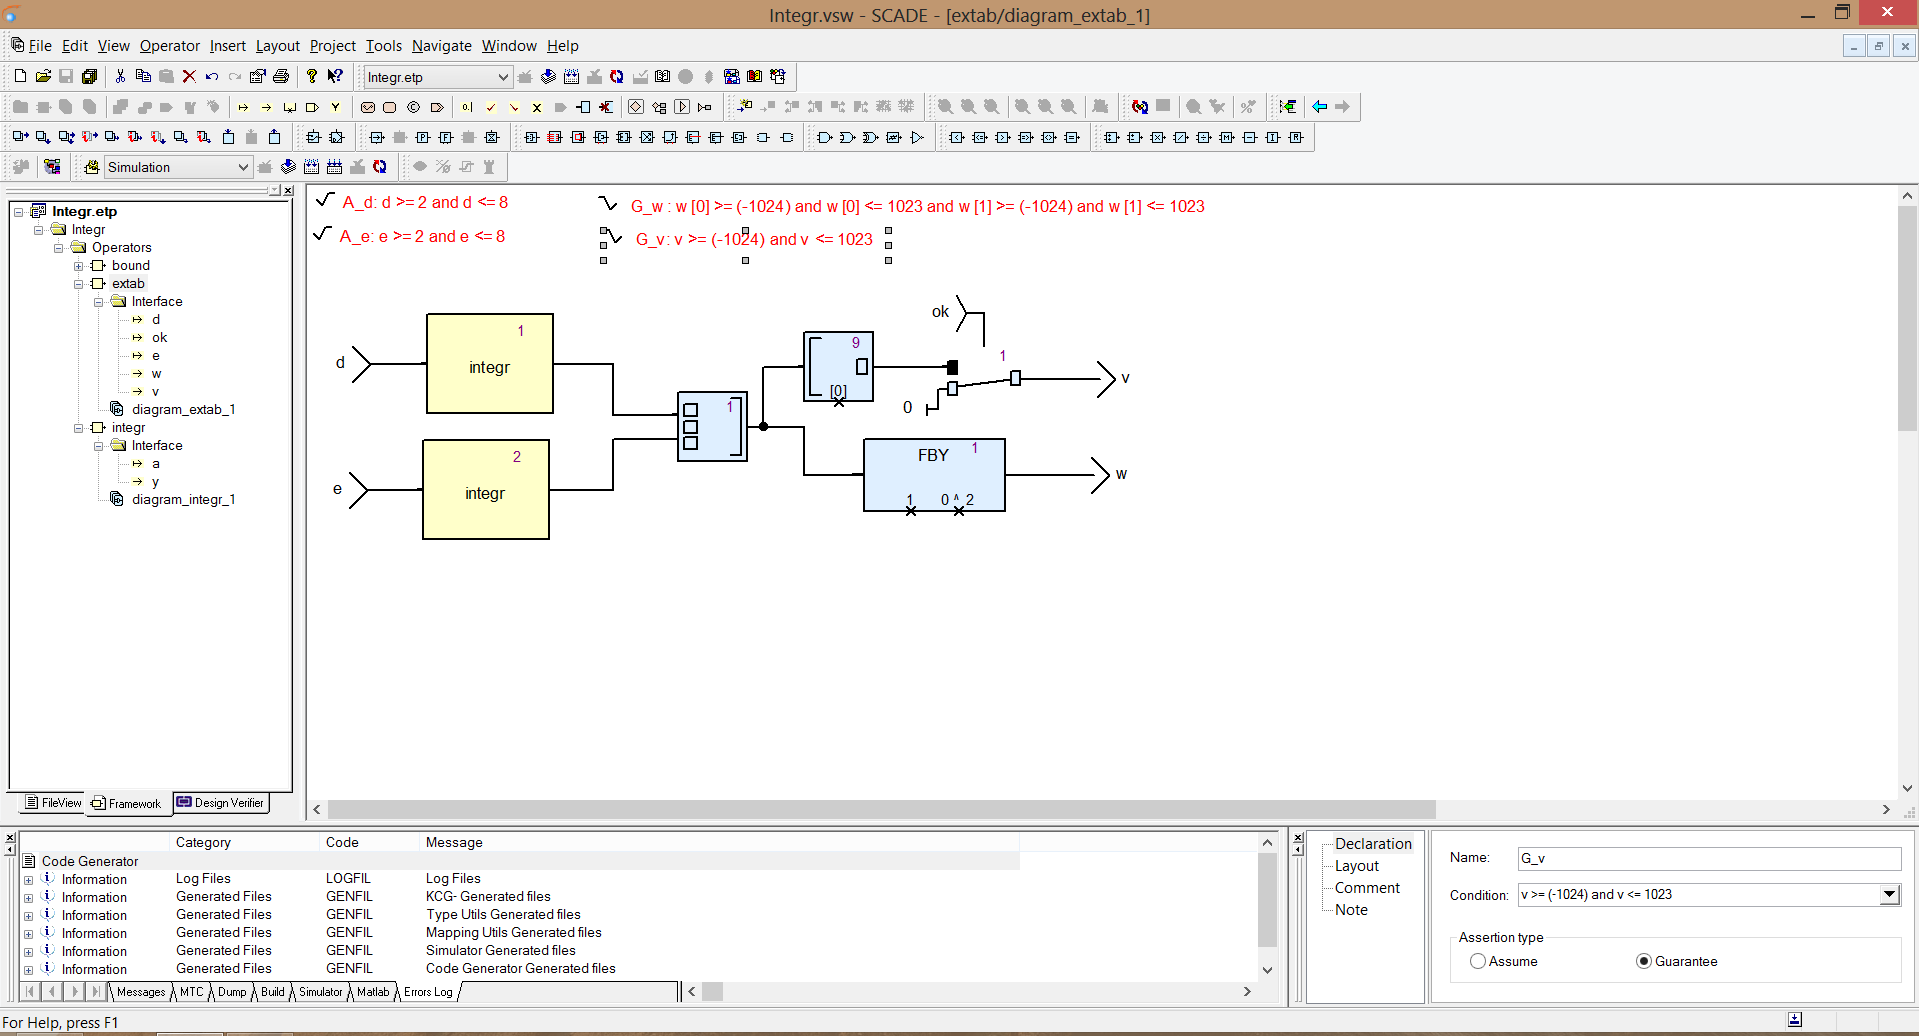
\includegraphics[scale=0.30]{1_scade.png}
\end{frame}
\begin{frame}
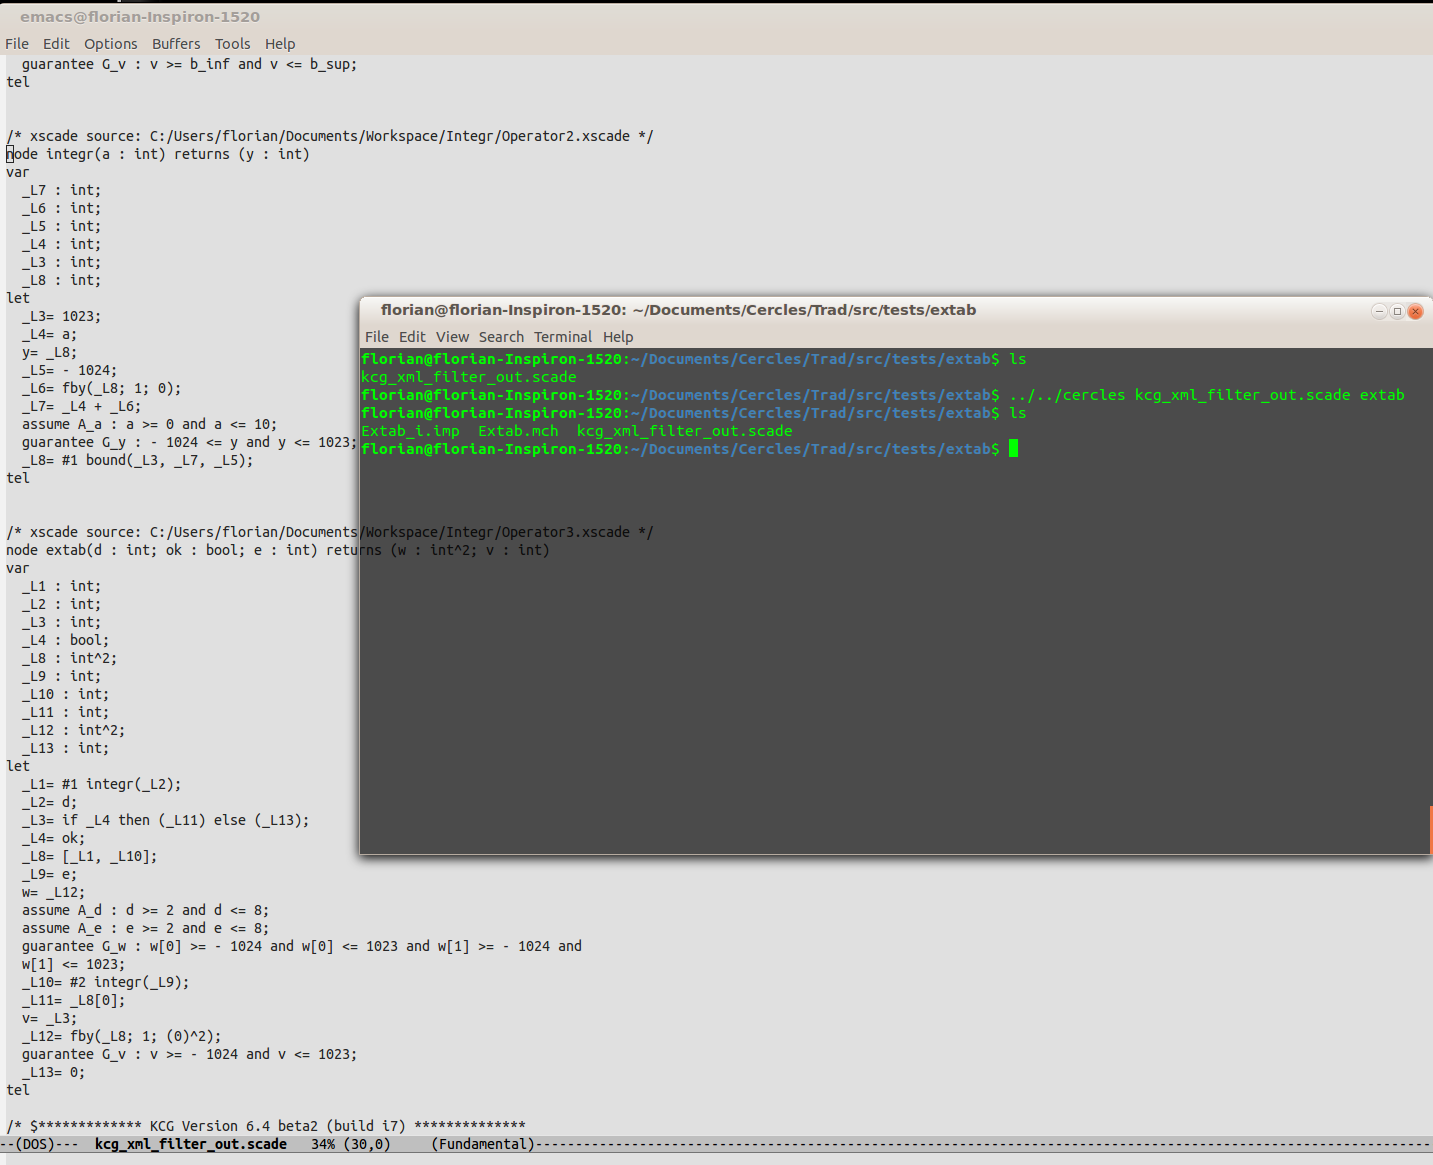
\includegraphics[scale=0.23]{2_term.png}
\end{frame}
\begin{frame}
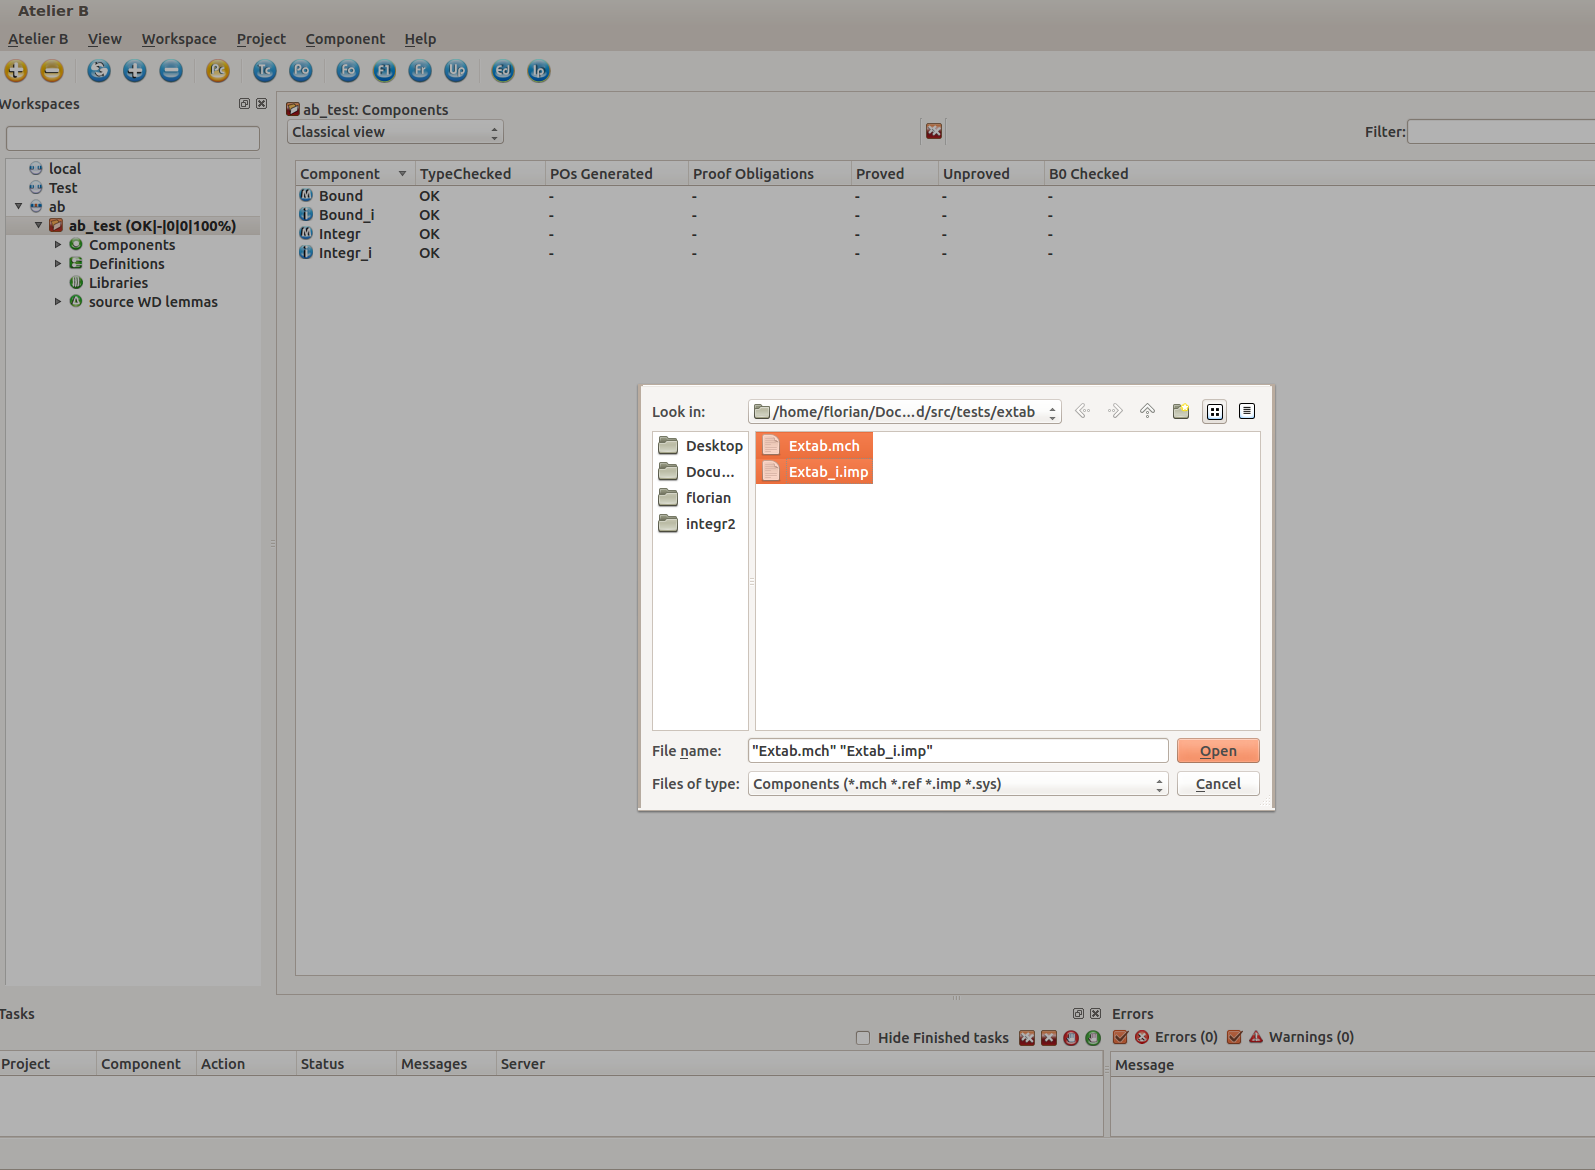
\includegraphics[scale=0.23]{3_open.png}
\end{frame}
\begin{frame}
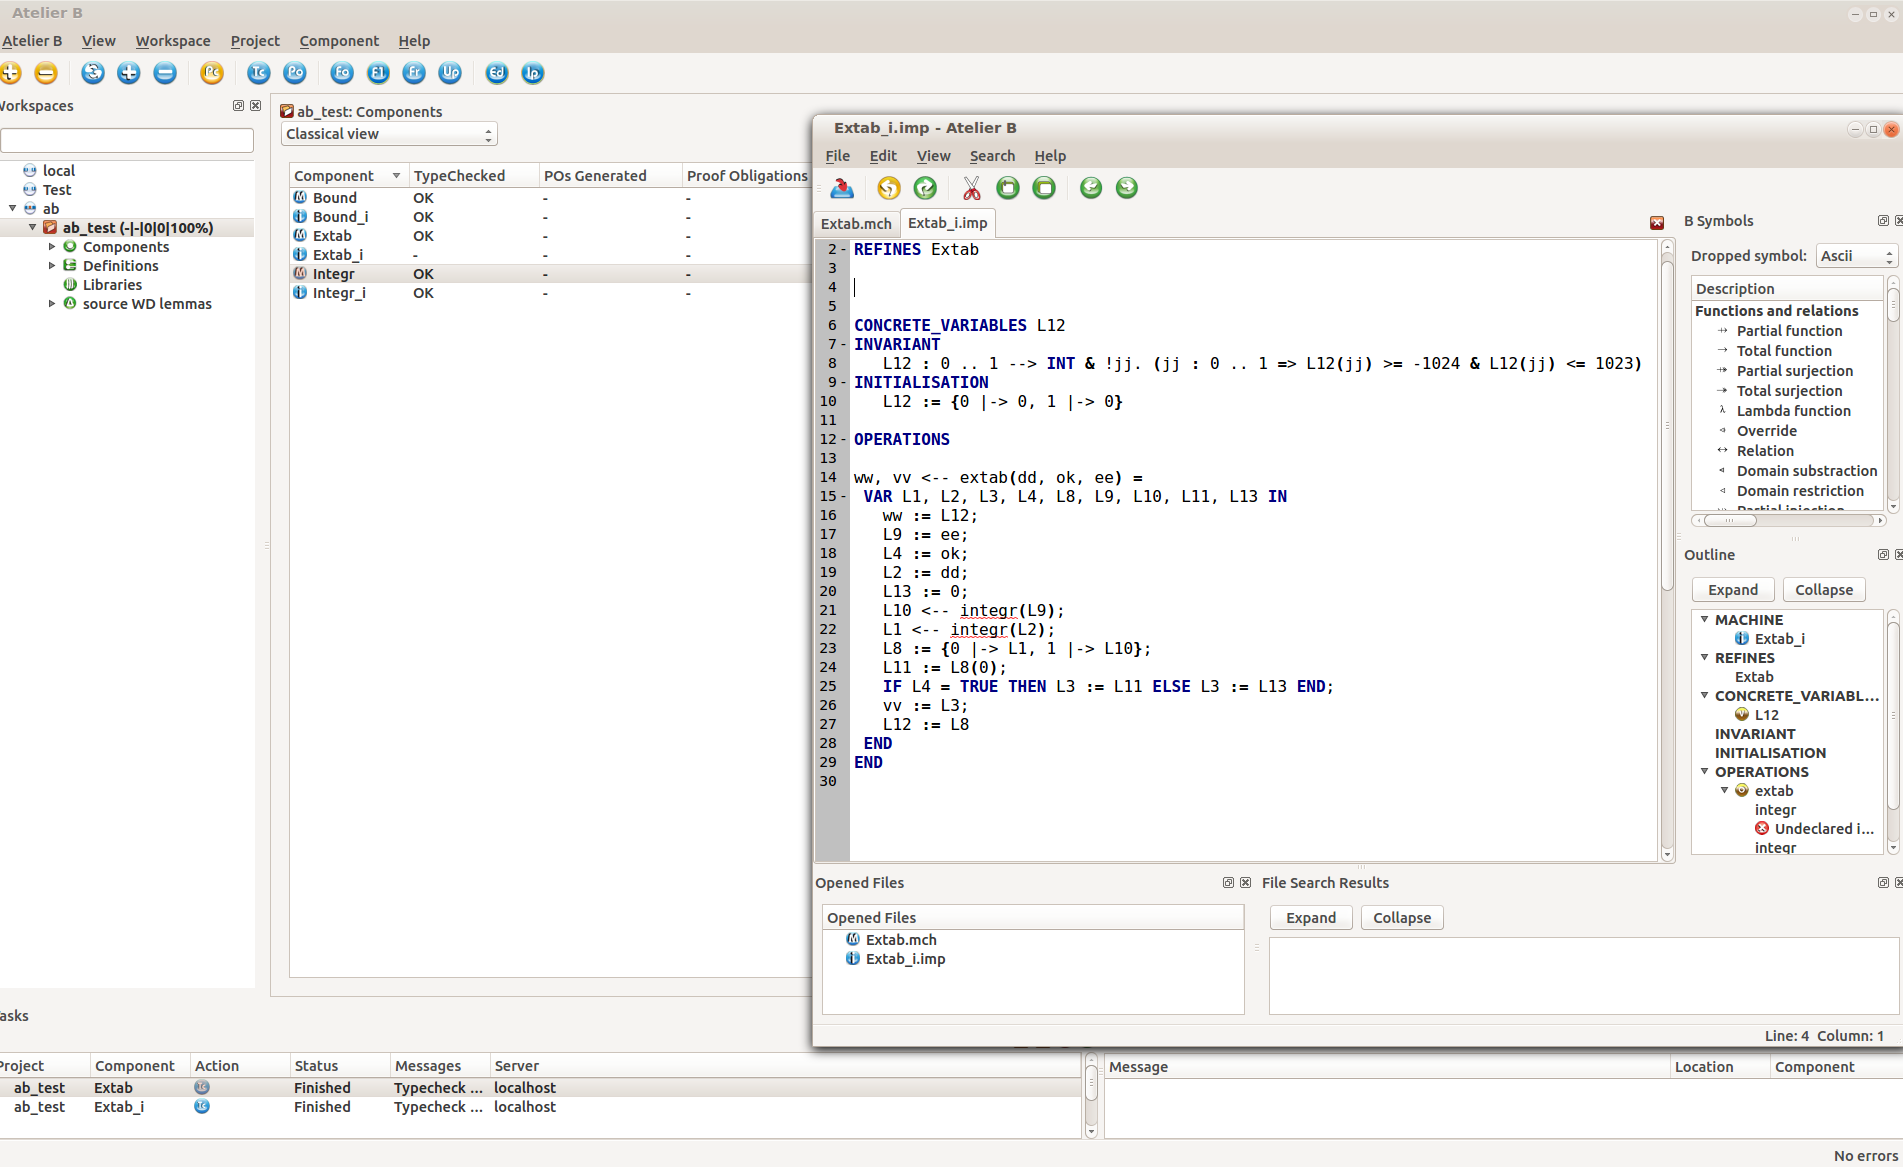
\includegraphics[scale=0.18]{4_integ.png}
\end{frame}
\begin{frame}
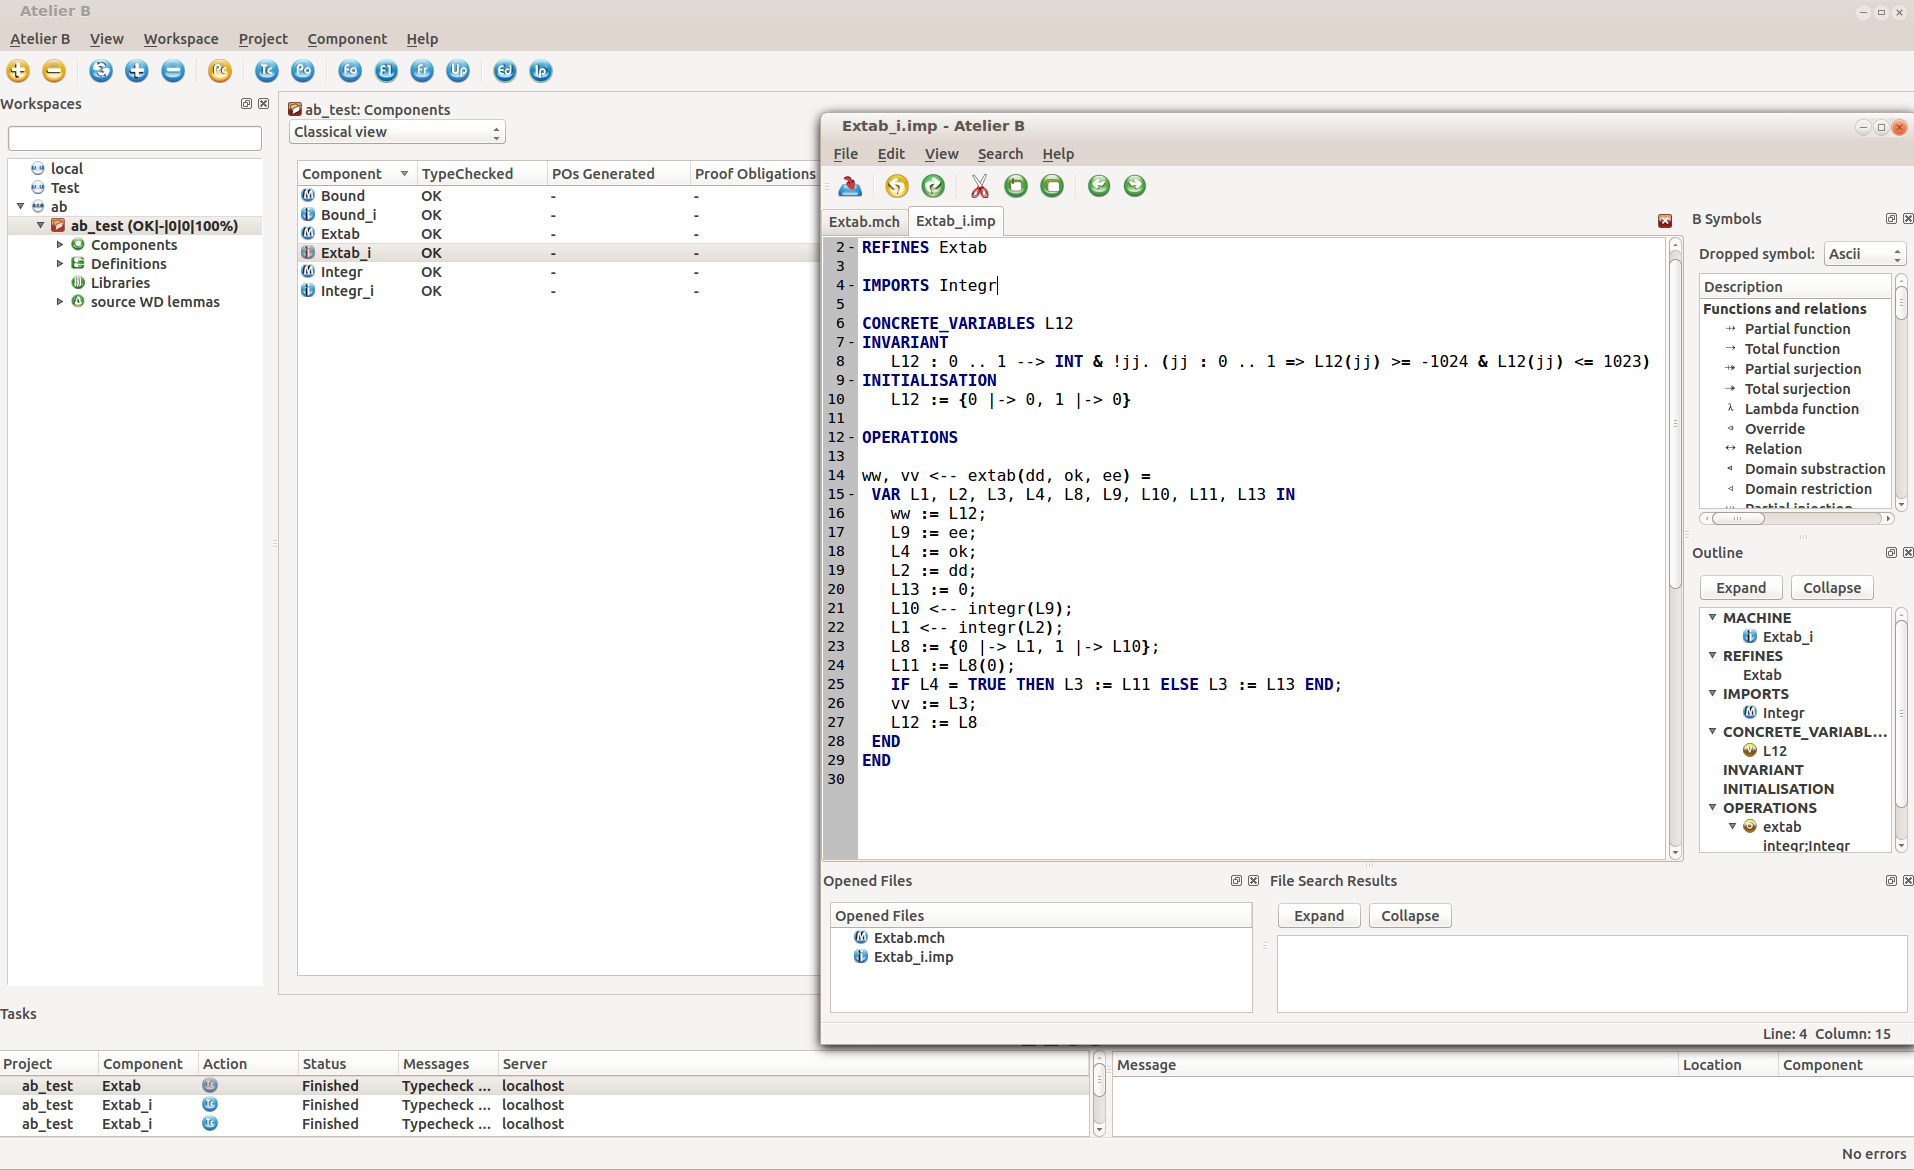
\includegraphics[scale=0.18]{5_ok.png}
\end{frame}
\begin{frame}
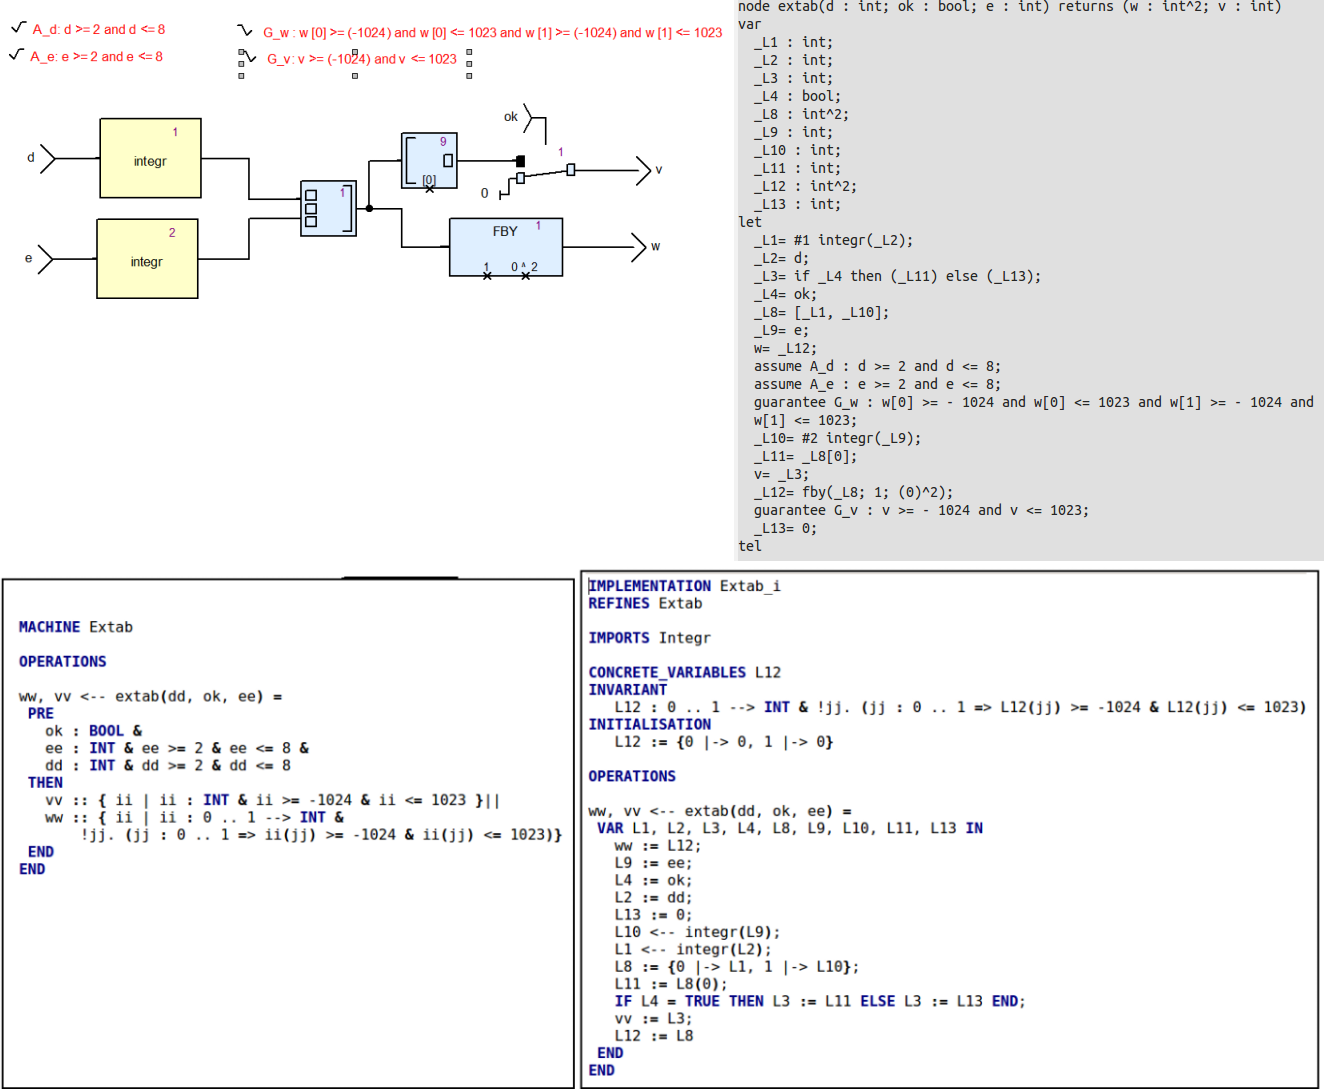
\includegraphics[scale=0.23]{final2.png}
\end{frame}


\section{Conclusion}
\frame{\sectionpage}
\begin{frame}

Traducteur fonctionnel, respecte les schémas de traduction.

\vspace{1cm}
\uncover<2->{
Fragment de Scade. Possibilités d'extensions \textbf{?}
}

\vspace{1cm}

\uncover<3->{
Preuve de correction de la traduction à faire.
}

\vspace{1cm}

\uncover<4->{
Remplacement des tests de composants par une étape de validation par méthode formelle \textbf{??}
}


\end{frame}

\begin{frame}
\begin{huge}
Merci de votre attention.
\end{huge}
\end{frame}


\end{document}
